\documentclass{beamer}\usepackage[]{graphicx}\usepackage[]{color}
%% maxwidth is the original width if it is less than linewidth
%% otherwise use linewidth (to make sure the graphics do not exceed the margin)
\makeatletter
\def\maxwidth{ %
  \ifdim\Gin@nat@width>\linewidth
    \linewidth
  \else
    \Gin@nat@width
  \fi
}
\makeatother

\definecolor{fgcolor}{rgb}{0.345, 0.345, 0.345}
\newcommand{\hlnum}[1]{\textcolor[rgb]{0.686,0.059,0.569}{#1}}%
\newcommand{\hlstr}[1]{\textcolor[rgb]{0.192,0.494,0.8}{#1}}%
\newcommand{\hlcom}[1]{\textcolor[rgb]{0.678,0.584,0.686}{\textit{#1}}}%
\newcommand{\hlopt}[1]{\textcolor[rgb]{0,0,0}{#1}}%
\newcommand{\hlstd}[1]{\textcolor[rgb]{0.345,0.345,0.345}{#1}}%
\newcommand{\hlkwa}[1]{\textcolor[rgb]{0.161,0.373,0.58}{\textbf{#1}}}%
\newcommand{\hlkwb}[1]{\textcolor[rgb]{0.69,0.353,0.396}{#1}}%
\newcommand{\hlkwc}[1]{\textcolor[rgb]{0.333,0.667,0.333}{#1}}%
\newcommand{\hlkwd}[1]{\textcolor[rgb]{0.737,0.353,0.396}{\textbf{#1}}}%

\usepackage{framed}
\makeatletter
\newenvironment{kframe}{%
 \def\at@end@of@kframe{}%
 \ifinner\ifhmode%
  \def\at@end@of@kframe{\end{minipage}}%
  \begin{minipage}{\columnwidth}%
 \fi\fi%
 \def\FrameCommand##1{\hskip\@totalleftmargin \hskip-\fboxsep
 \colorbox{shadecolor}{##1}\hskip-\fboxsep
     % There is no \\@totalrightmargin, so:
     \hskip-\linewidth \hskip-\@totalleftmargin \hskip\columnwidth}%
 \MakeFramed {\advance\hsize-\width
   \@totalleftmargin\z@ \linewidth\hsize
   \@setminipage}}%
 {\par\unskip\endMakeFramed%
 \at@end@of@kframe}
\makeatother

\definecolor{shadecolor}{rgb}{.97, .97, .97}
\definecolor{messagecolor}{rgb}{0, 0, 0}
\definecolor{warningcolor}{rgb}{1, 0, 1}
\definecolor{errorcolor}{rgb}{1, 0, 0}
\newenvironment{knitrout}{}{} % an empty environment to be redefined in TeX

\usepackage{alltt}

\mode<presentation> {

% The Beamer class comes with a number of default slide themes
% which change the colors and layouts of slides. Below this is a list
% of all the themes, uncomment each in turn to see what they look like.

%\usetheme{default}
\usetheme{AnnArbor}
%\usetheme{Antibes}
%\usetheme{Bergen}
%\usetheme{Berkeley}
%\usetheme{Berlin}
%\usetheme{Boadilla}
%\usetheme{CambridgeUS}
%\usetheme{Copenhagen}
%\usetheme{Darmstadt}
%\usetheme{Dresden}
%\usetheme{Frankfurt}
%\usetheme{Goettingen}
%\usetheme{Hannover}
%\usetheme{Ilmenau}
%\usetheme{JuanLesPins}
%\usetheme{Luebeck}
%\usetheme{Madrid}
%\usetheme{Malmoe}
%\usetheme{Marburg}
%\usetheme{Montpellier}
%\usetheme{PaloAlto}
%\usetheme{Pittsburgh}
%\usetheme{Rochester}
%\usetheme{Singapore}
%\usetheme{Szeged}
%\usetheme{Warsaw}

% As well as themes, the Beamer class has a number of color themes
% for any slide theme. Uncomment each of these in turn to see how it
% changes the colors of your current slide theme.

%\usecolortheme{albatross}
%\usecolortheme{beaver}
%\usecolortheme{beetle}
%\usecolortheme{crane}
%\usecolortheme{dolphin}
%\usecolortheme{dove}
%\usecolortheme{fly}
\usecolortheme{lily}
%\usecolortheme{orchid}
%\usecolortheme{rose}
%\usecolortheme{seagull}
%\usecolortheme{seahorse}
%\usecolortheme{whale}
%\usecolortheme{wolverine}

%\setbeamertemplate{footline} % To remove the footer line in all slides uncomment this line
\setbeamertemplate{footline}[page number] % To replace the footer line in all slides with a simple slide count uncomment this line

%\setbeamertemplate{navigation symbols}{} % To remove the navigation symbols from the bottom of all slides uncomment this line
}

\usepackage{graphicx} % Allows including images
\usepackage{booktabs} % Allows the use of \toprule, \midrule and \bottomrule in tables

%----------------------------------------------------------------------------------------
%	TITLE PAGE
%----------------------------------------------------------------------------------------

\title[The Importance of Documenting Where Your Data is From]{DOCUMENT EVERYTHING} % The short title appears at the bottom of every slide, the full title is only on the title page

\author{Maureen O'Donnell} % Your name
\institute[4870] % Your institution as it will appear on the bottom of every slide, may be shorthand to save space
{
Dr. Arnholt Senior Seminar\\ % Your institution for the title page
\medskip
\textit{odonnellm@appstate.edu} % Your email address
}
\date{\today} % Date, can be changed to a custom date
\IfFileExists{upquote.sty}{\usepackage{upquote}}{}

\begin{document}

\begin{frame}
\titlepage % Print the title page as the first slide
\end{frame}

\begin{frame}
\frametitle{Overview} % Table of contents slide, comment this block out to remove it
\tableofcontents % Throughout your presentation, if you choose to use \section{} and \subsection{} commands, these will automatically be printed on this slide as an overview of your presentation
\end{frame}

%----------------------------------------------------------------------------------------
%	PRESENTATION SLIDES
%----------------------------------------------------------------------------------------

%------------------------------------------------
\section{What To Document?} % Sections can be created in order to organize your presentation into discrete blocks, all sections and subsections are automatically printed in the table of contents as an overview of the talk
%------------------------------------------------

\subsection{Where did you get the data?} % A subsection can be created just before a set of slides with a common theme to further break down your presentation into chunks

\begin{frame}
\frametitle{Where did you get the data?}
The location of where your data is from is very important to document.  In the data frame used in the NC Voter project had 4 sources of data. As you will soon see we did not document the data well.\\~\\

When documenting where your data is from, be sure to include how you got it.  Did you have to click on multiple tabs within the page? Was it a direct url? How often is the data changed?
\end{frame}

%------------------------------------------------

\begin{frame}
\frametitle{Where Our Data Was From}
\begin{itemize}
\item NC Voter Info Site
\begin{itemize}
\item Easiest site to use of the bunch
\end{itemize}
\item US Census Bureau
\begin{itemize}
\item Not a good idea to use this site. In fact DO NOT use it.  It is miserable to search through and very hard to find a simple file.
\end{itemize}
\item Two Church sites
\begin{itemize}
\item Not as bad to use.  However we did not document the location within the site so finding the data has proved difficult.
\end{itemize}
\item North Carolina Education site
\begin{itemize}
\item Also not to bad to use. Again we did not document where in the site the data was.
\end{itemize}
\end{itemize}
\end{frame}

%------------------------------------------------

\begin{frame}
\frametitle{URL's of the sites we used}
\begin{block}{NC Voter}
http://www.ncsbe.gov/
\end{block}

\begin{block}{Census}
http://factfinder2.census.gov
\end{block}

\begin{block}{Churches}
http://www.thearda.com
\end{block}

\begin{block}{Education}
http://collegestats.org/colleges/north-carolina
\end{block}
\end{frame}

%------------------------------------------------
\subsection{How to Store the Data?}
%------------------------------------------------

\begin{frame}
\frametitle{How to Store the Data}

\begin{itemize}
\item Pick one place for all group members to store the data
\item Don't use 1 billion different locations to store the data, like we did.
\item Label any changes you make so all the group can see.
\item Date all changes
\end{itemize}
\end{frame}

%------------------------------------------------
\section{Our Project}
%------------------------------------------------

\begin{frame}
\frametitle{Screen Shot 1}
\begin{figure}[ht!]
\centering
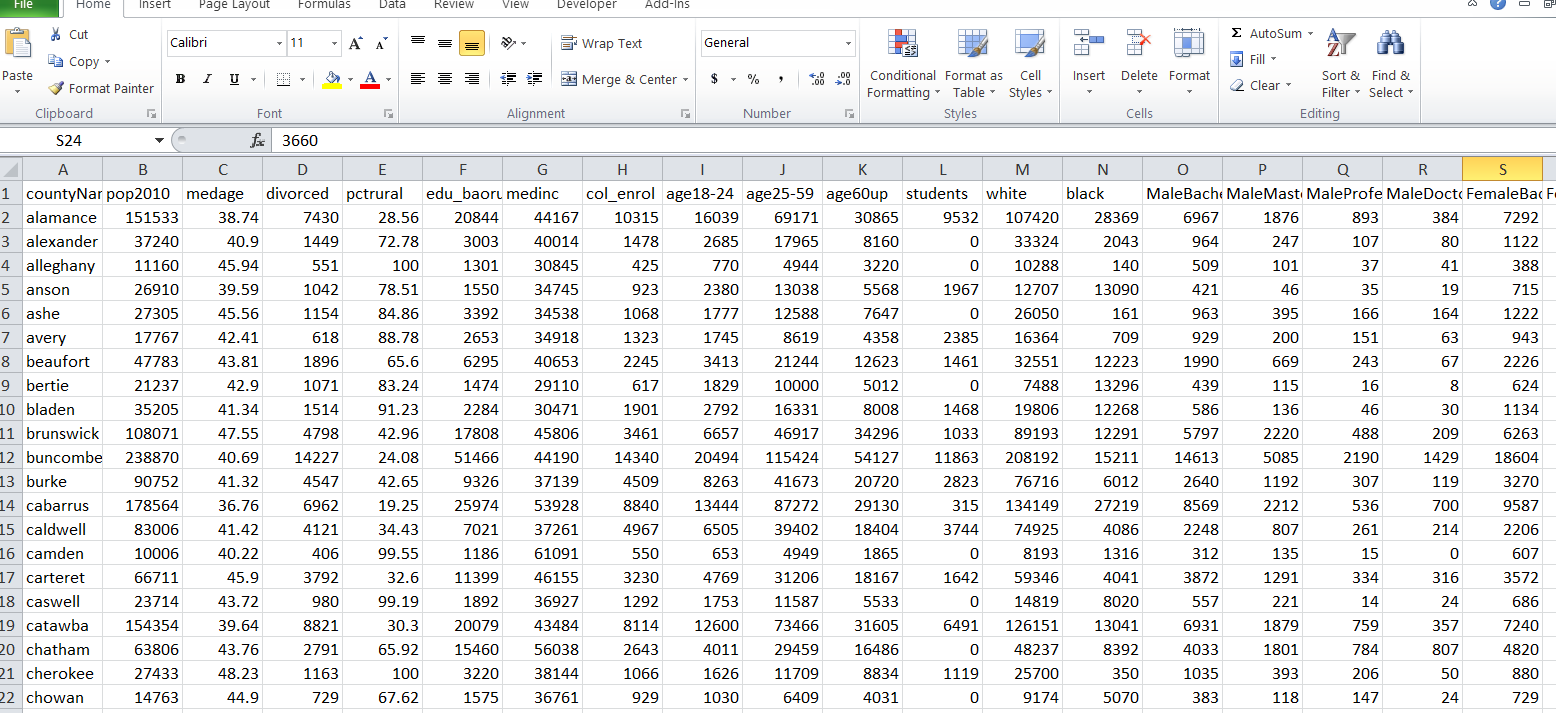
\includegraphics[width=90mm]{excel.jpeg}
\caption{A portion of our data}
\label{Data}
\end{figure}
\end{frame}

%------------------------------------------------

\begin{frame}
\frametitle{Screen Shot 2}
\begin{figure}[ht!]
\centering
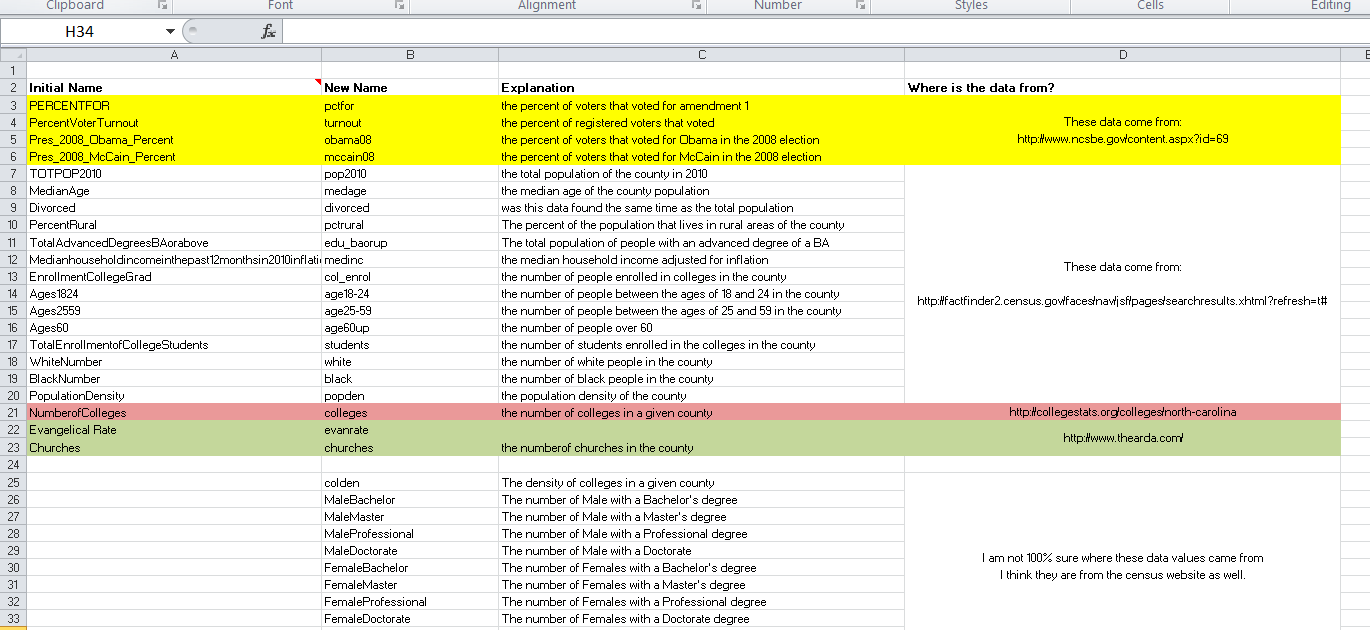
\includegraphics[width=90mm]{variable.jpeg}
\caption{Our variable table}
\label{Variable}
\end{figure}
\end{frame}

%------------------------------------------------

\begin{frame}
\frametitle{Screen Shot 3}
\begin{figure}[ht!]
\centering
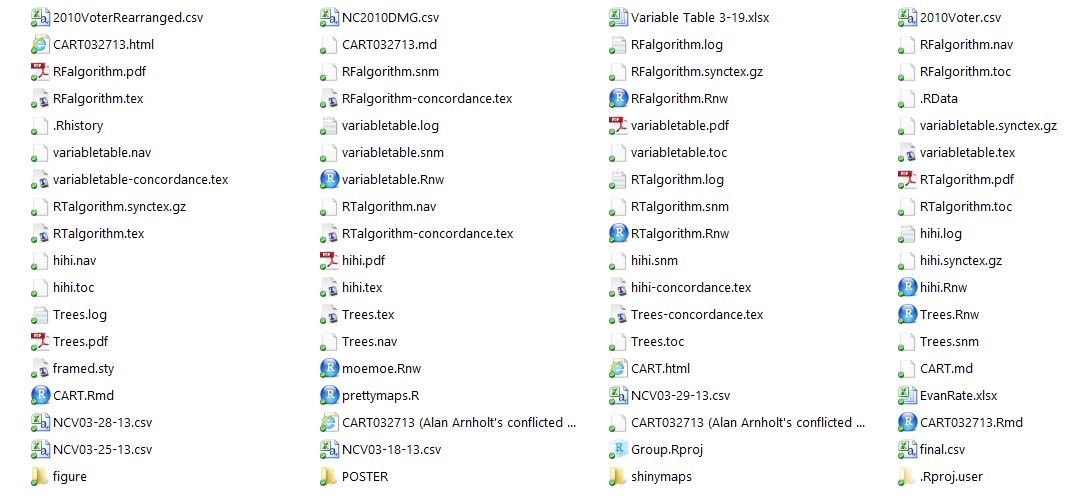
\includegraphics[width=90mm]{groupfolder.jpg}
\caption{One of our messy folders}
\label{Group Folder}
\end{figure}
\end{frame}

%------------------------------------------------
\section{In Summary}

\begin{frame}
\frametitle{What to take away}
Large data sets can seem difficult to manage but with appropriate storage techniques it can be quite easy. 
\\~\\

Once all the data is stored the resulting R package will use what you've done to make is user friendly to anyone wishing to do analysis with it.

%\begin{figure}
%\includegraphics[width=0.8\linewidth]{test}
%\end{figure}
\end{frame}

%------------------------------------------------


\begin{frame}
\Huge{\centerline{The End}}
\end{frame}

%----------------------------------------------------------------------------------------

\end{document} 
